\section{问题背景与问题重述}

\subsection{问题背景}

随着分布式光伏的接入，光伏出力与小区负载在时间上的峰谷错位使传统供电调节方式难以胜任。
非孤岛式微网把小区负载、分布式电源与储能设备整合为一个可调的小型发用电系统，
通过在外网电价低时充电、高时放电获取经济效益，是消纳分布式能源的关键技术。

微网调控的难点在于：外网电价分时波动、光伏出力难以精确预测、储能又受容量与充放电功率双重约束。
在保证供电的前提下最小化购电支出，因而是一个受多方面约束的动态优化决策问题；
当计划购电与实际执行出现偏差时还会产生高价的紧急购电费与违约费，进一步提高了问题的复杂度。
因此需要建立一套可操作的微网与外部电网电力调控策略，在电价波动与预测误差下动态调整每日购电计划。

\subsection{问题重述}

题目由确定性调度逐步扩展到预测不确定性、日内信息更新与实时电价波动四个层次。

\textbf{问题一：} 每日电价与小区负载相同、已给出一天的光伏预测功率，需在每天 0:00 制定全天计划购电策略，
要求任意时段供电不少于负载，且 0:00 与 24:00 储电量相同，并给出计划购电量、充放电量与购电费用。

\textbf{问题二：} 电价规律相同而负荷、光伏随日期变化，需在每天 0:00 提前制定全天计划购电量；
若实际供电不足，按交易时刻电价的 5 倍紧急购电，因此需在正常购电成本与紧急补救风险之间权衡。

\textbf{问题三：} 在问题二基础上，每天 0:00、6:00、12:00、18:00 均可获得未来 24 h 的新光伏预报，
允许对尚未执行时段调整计划购电量：调增按 1.5 倍电价结算，调减承担 0.5 倍电价违约成本；
需建立利用新预报滚动修正的策略，并分析增加预报时点是否有必要。

\textbf{问题四：} 进一步考虑外网实时电价本身随时间波动。在未来真实电价不可提前获知的条件下，
需对问题二、三的模型增加电价预测与价格不确定性处理，重新得到波动电价下的计划购电与滚动调整策略。

四问的建模主线与数据流如图~\ref{fig:flow} 所示：从确定性的能量分流调度出发，
依次引入预测误差下的日前随机决策、多时点信息更新下的日内再决策，最后纳入实时电价不确定性；
后一问在前一问的模型结构上叠加一层新信息，物理约束与决策变量体系保持连续，四问构成递进关系。

\begin{figure}[htbp]
\centering
% 流程图按原始比例放大展示，不设高度上限（缩小会看不清）
% trim 参数为 左 下 右 上；原图上下各约 8%/9% 是纯白边，裁掉不影响内容
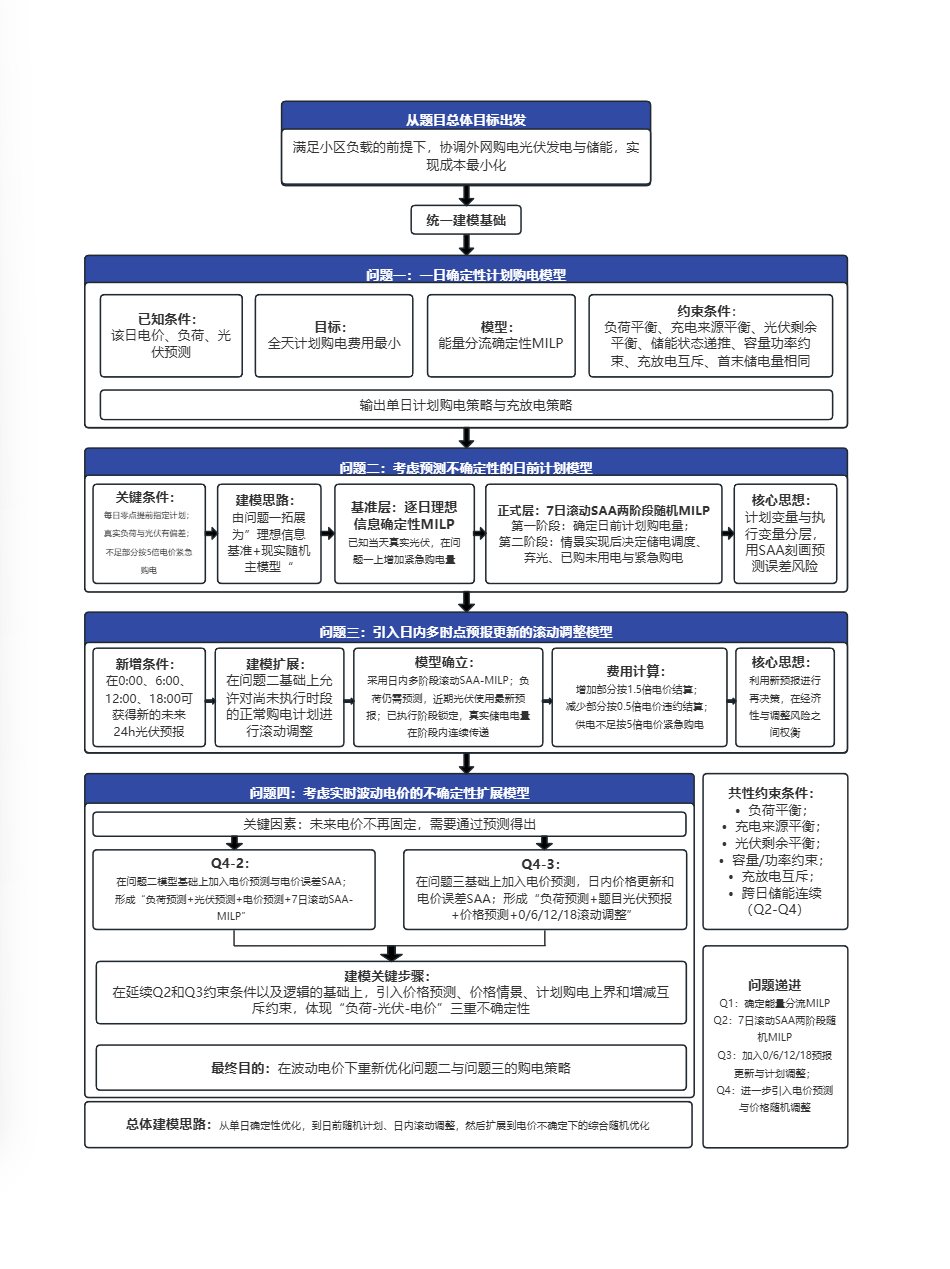
\includegraphics[width=0.86\textwidth,trim=0 120 101 100,clip]{figures/flowchart.png}
\caption{微网购电调控的总体建模流程}
\label{fig:flow}
\end{figure}
